\section{Technical acknowledgements}
\paragraph{}
The following code presented was written using \emph{R}. The images from which the shapes were extracted were used as gray images. \ref{fig:gray-images}

\section{Loading data}
\paragraph{}
In the first phase, we'll be working with files containing pre-defined contour points.
These are just pairs $(x, y)$ representing the coordinates of the outer points of a shape's contour.
To simplify things, we'll transform the coordinates to complex numbers: \cite{complex_number}.

\begin{lstlisting}[language=R, caption=Loading outer contour points]
    # Lit un contour dans un fichier texte
    rdfChargeFichierContour <- function (nom) {
        contour <- read.table (nom)
        complex (real = contour$V1, imaginary = contour$V2)
    }
\end{lstlisting}

\paragraph{}
Images used are loaded then converted to grayscale. Right now, we are not interested in their color, so they'll only be black and white.

\begin{lstlisting}[language=R, caption=Loading images]
    rdfReadGreyImage <- function (nom) {
        image <- readImage (paste('images/', nom, sep=''))
        if (length (dim (image)) == 2) {
            image
        } else {
            channel (image, 'red')
        }
    }
\end{lstlisting}

\begin{figure}[ht]
    \centering
    
\includegraphics[scale=2.0]{rdf-carre-20.png}
    
\includegraphics[scale=2.0]{rdf-croix.png}
    
\includegraphics[scale=2.0]{rdf-patate.png}
    
\includegraphics[scale=2.0]{rdf-triangle-20.png}
    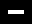
\includegraphics[scale=2.0]{rdf-rectangle-horizontal.png}
    \caption{Shape images}
    \label{fig:gray-images}
\end{figure}

\clearpage

\section{Fourier Descriptors}
\subsection{Outer contour points}
\paragraph{}
Let's take a look at how one of our initial shape looks like. The red contour contains all of our points.
The blue one is drawn between each 4th point, and the green one is drawn between each 8th point.
\begin{figure}[ht]
    \centering
    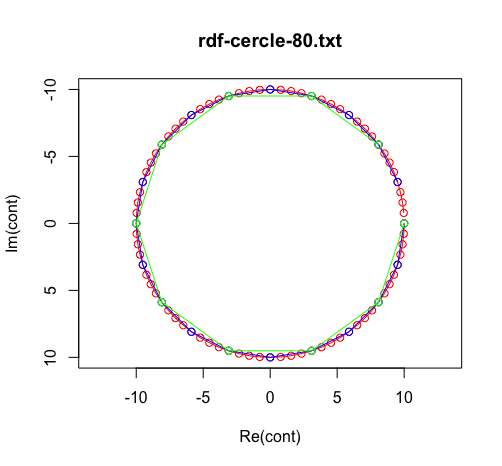
\includegraphics[width=\textwidth]{rdf-cercle-contour.png}
    \caption{Circle contour}
\end{figure}

\paragraph{}
If we apply the \emph{Fast Fourier Transform} on our contour points, we'll get our \emph{Fourier descriptors}\footnote{The Fourier descriptors were normalised by dividing them to the length of the total contour points}.
We can use these to describe our contour and we're even able to reconstruct our contour starting from fourier descriptors.

\begin{lstlisting}[language=R, caption=Calculating Fourier descriptors]
    reconstructShapeWithFourier <- function(nom){
        cont <- rdfChargeFichierContour(nom)
        fourier <- fft(cont)/length(cont)
        inversed <- fft(fourier, inverse=TRUE)
        print ("Can we reconstruct our shape from Fourier descriptors?")
        print (all.equal(inversed, cont))
    }
\end{lstlisting}

\paragraph{}
Here's how the Fourier descriptors look like calculated on the contour of the square:
\begin{figure}[ht]
    \centering
    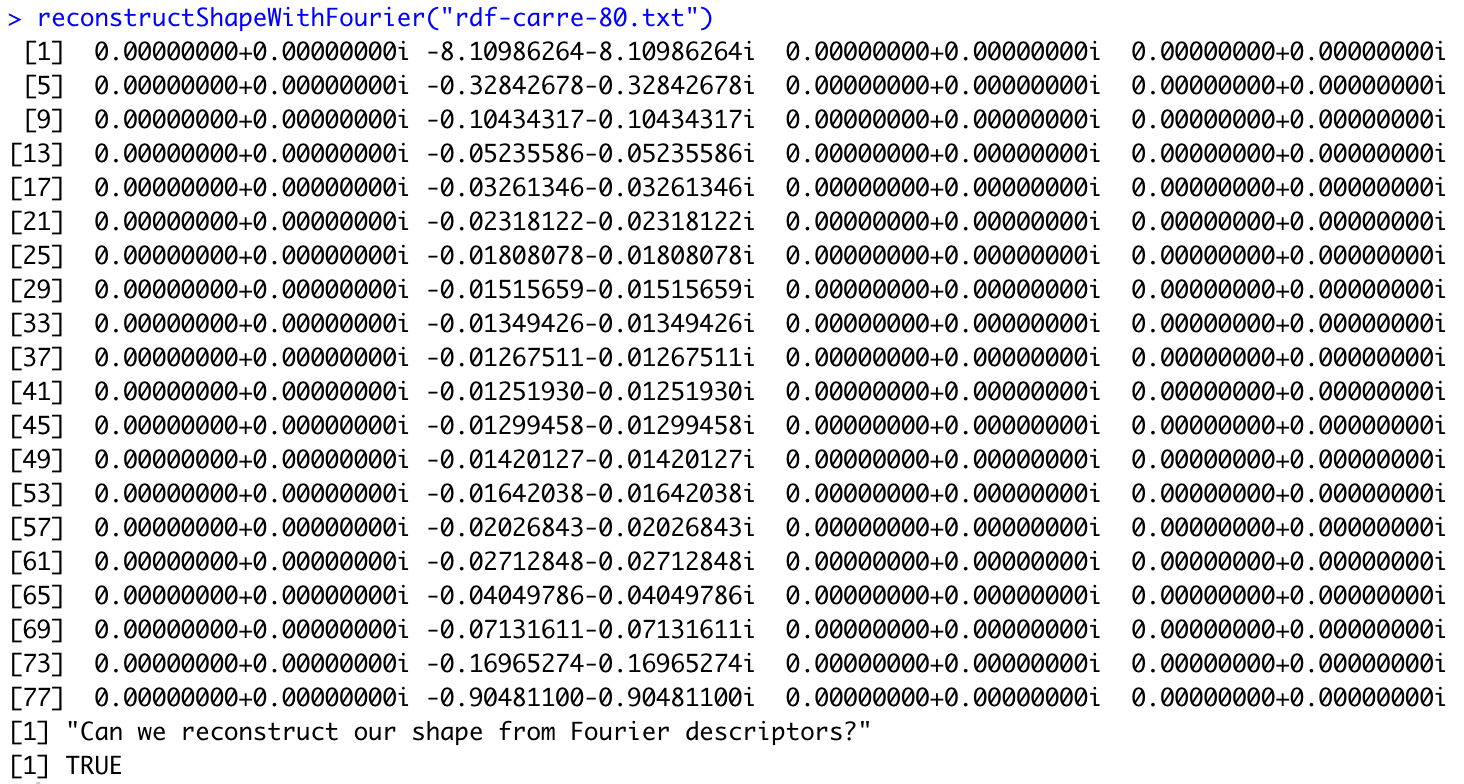
\includegraphics[width=\textwidth]{fourier_descriptors.png}
    \caption{Reconstructing contour from Fourier descriptors}
\end{figure}

\paragraph{}
As we can see, we can safely reconstruct our initial contour thanks to the \emph{Inverse Fast Fourier Transform}: \cite[FFT]{fast_fourier_transform}.
An interesting observation is that the first Fourier descriptor, $Z_0$, represents the center of the shape.
If we modify this complex number (for example $Z_0 = Z_0 + 0.5 + 3i$) we'll actually do a \emph{translation}.

\begin{figure}[ht]
    \centering
    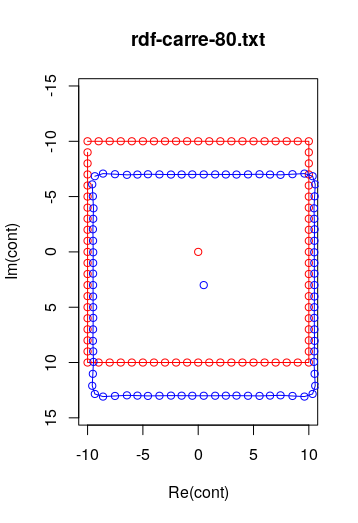
\includegraphics[scale=0.6]{center_shift.png}
    \caption{Modifying $Z_0$}
\end{figure}

\clearpage

\subsection{Cancelling Fourier descriptors}
\paragraph{}
We can simplify our contour by ``cancelling'' some of the Fourier descriptors.
We can do so by defining a \emph{ratio} of descriptors that we'd like to keep.
When doing so, it is important to know that we should start cancelling the descriptors from the middle of the descriptor list: \cite[RDF Course]{lille_rdf_course}.

\begin{lstlisting}[language=R, caption=Simplifying contour]
    rdfAnnuleDescFourier <- function (desc, ratio){
        if (ratio == 1.0)
            desc
        
        nb_delete <- length(desc) - length(desc) * ratio
        middle <- length(desc)/2
        start <- middle - nb_delete/2
        end <- middle + nb_delete/2
        desc[start:end] <- 0
        desc
    }
\end{lstlisting}

\begin{figure}[ht]
    \centering
    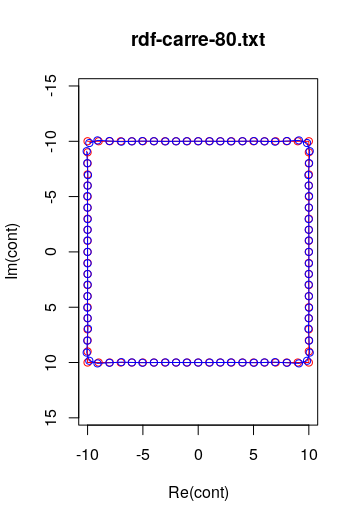
\includegraphics[width=\textwidth/2-10pt]{fourier_simplified_1.png}
    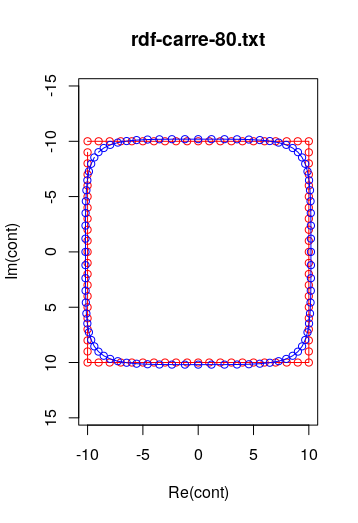
\includegraphics[width=\textwidth/2-10pt]{fourier_simplified_2.png}
    \caption{Cancelling Fourier descriptors, $ratio \in \{0.5, 0.075\}$}
\end{figure}

\clearpage

\section{Simplifying the shape contour}
\paragraph{}
We can make use of \emph{circle's chord} to reduce the number of outer contour points. We'll reduce our shape to a sequence of segments between points.
Given a sequence of contour points $S = P_1, \dots, P_n$ and $P_1P_n$ the line between the first and last point, we define $X$ as the "furthest" point from this line and $d_X$ the distance from $X$ to $P_1P_n$.
If $d_X$ is less than some $d_{max}$, then we add the segment $P_1P_n$ as part of our ``simplified'' contour.
If not, we divide $S$ into $S_1 = P_1, \dots, X$ and $S_2 = X, \dots, P_n$ and apply the same algorithm as above.
Please refer to \cite{point_to_line_distance} and \cite{line_equation_complex_numbers} for how the distances were calculated.

\begin{lstlisting}[language=R, caption=Chord algorithm]
    # Algorithme de la corde pour la reduction d'un contour
    rdfAlgorithmeCorde <- function (cont, dmax) {
        # Calcul des distances
        d <- rdfDistances (cont)
        # Si distance maxi inferieur au seuil, ne garder que les extremites
        if (max (d) <= dmax) {
            c (head (cont, 1), tail (cont, 1))
        # Sinon decouper en deux parties
        } else {
            # Point le plus eloigne
            loin <- which.max (d)
            # Reduire les deux sous chaines
            cont1 <- rdfAlgorithmeCorde (cont[1:loin], dmax)
            cont2 <- rdfAlgorithmeCorde (cont[loin:length (cont)], dmax)
            # Enlever un point et contatener
            c (cont1, tail (cont2, -1))
        }
    }
\end{lstlisting}

\begin{lstlisting}[language=R, caption=Calculating distances from $P_1P_n$ to each point]
    # Calcul des distances entre les points et la corde
    rdfDistances <- function (cont) {
        # Points extremes
        debut = head (cont, 1)
        fin = tail (cont, 1)
        distances <- rep (0, length (cont))
        for (i in 1:length(cont)){
            distances[i] <- rdfDistanceToLine(cont[i], debut, fin)
        }
        distances
    }
\end{lstlisting}

\begin{lstlisting}[language=R, caption=Distance from a point to a line]
    rdfDistanceToLine <- function (p, p1, p2){
        x1 <- Re(p1)
        y1 <- Im(p1)
        x2 <- Re(p2)
        y2 <- Im(p2)
        
        a <- y2 - y1
        b <- -(x2 - x1)
        c <- -x1*(y2 - y1) + y1*(x2-x1)
        
        res <- abs(a * Re(p) + b * Im(p) + c)/sqrt(a**2 + b**2)
        res
    }
\end{lstlisting}

\clearpage

\paragraph{}
Being able to parametrise the algorithm with $d_{max}$ will allow us to reach the trade-off between simplicity and precision that we mentioned in the introduction.\ref{trade-off}
Let's take a look at the results:
\begin{figure}[ht]
    \centering
    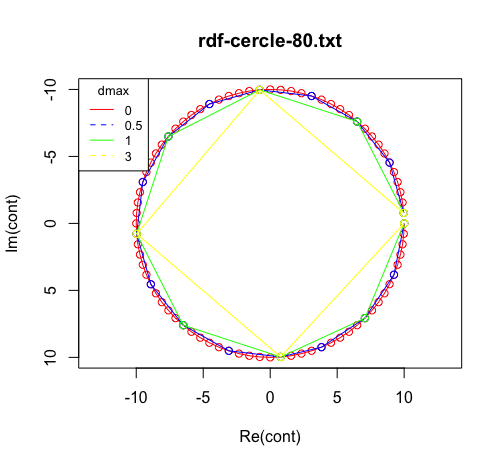
\includegraphics[width=\textwidth - 1pt]{chord_algorithm.png}
    \caption{Chord algorithm, $d_{max} \in \{0, 0.5, 1, 3\}$}
\end{figure}

\clearpage

\section{Fourier descriptors vs. Chord algorithm}
\paragraph{}
A natural question we may ask ourselves now is: which method is better?
Well, like in most Computer Science questions, the answer is the same: it depends.
Let's have a look at how each method can be used to describe the contour of a shape:

\begin{figure}[ht]
    \centering
    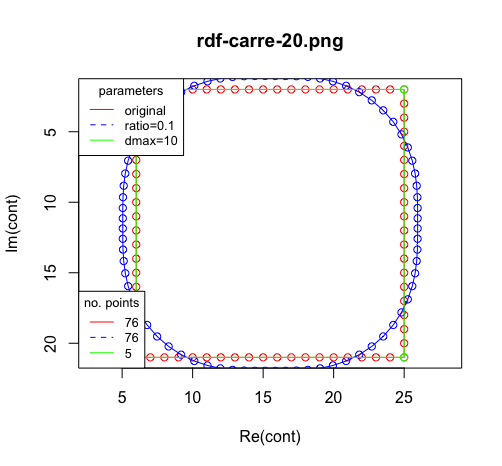
\includegraphics[width=\textwidth/2-50pt]{methods_carre.png}
    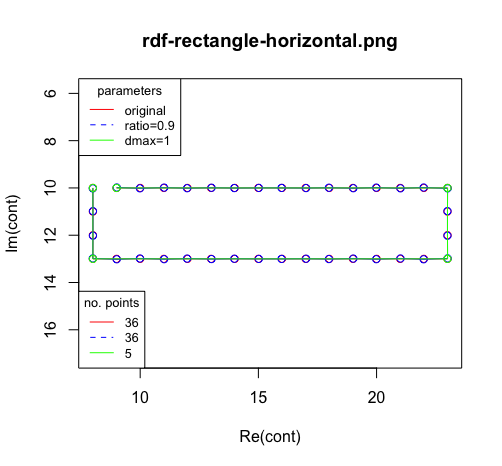
\includegraphics[width=\textwidth/2-50pt]{methods_rectangle.png}
    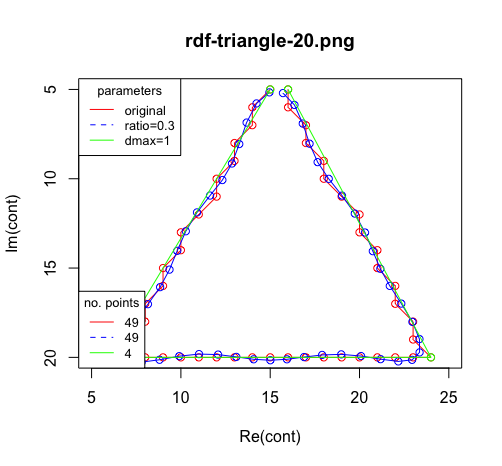
\includegraphics[width=\textwidth/2-50pt]{methods_triangle.png}
    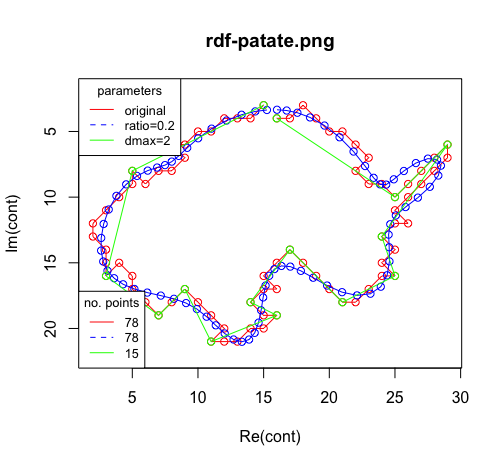
\includegraphics[width=\textwidth/2-50pt]{methods_patate.png}
    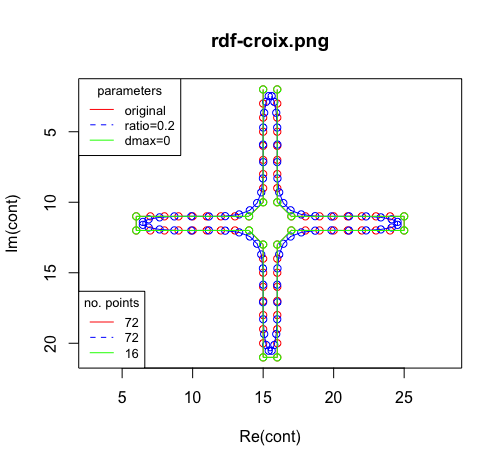
\includegraphics[width=\textwidth/2-50pt]{methods_croix.png}
    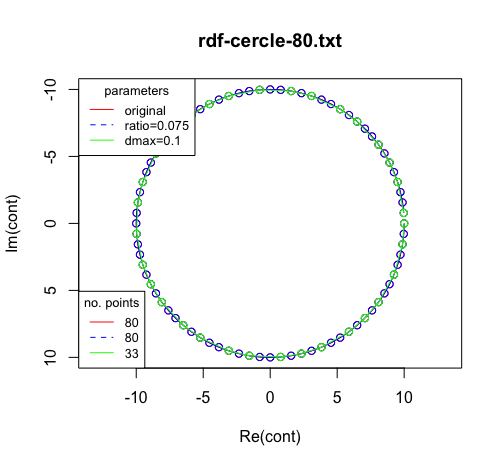
\includegraphics[width=\textwidth/2-50pt]{methods_cercle.png}
    \caption{Comparison between encoding methods}
    \label{methods-comparison}
\end{figure}

\clearpage

\paragraph{}
If we take a good look at the figures\ref{methods-comparison}, we can clearly see that the \emph{Chord Algorithm} is much better for shapes without curves.
For example, for the square and for the rectangle, we can reduce the initial number of points to just \emph{5}!
The same goes for triangle and the cross, where we can drastically reduce the number of points necessary.
\paragraph{}
Taking the rectangle as an example, the \emph{Fast Fourier Transform} method requires to keep around $90\%$ of the descriptors to be able to properly reconstruct the shape.
However, this method is much better for shapes with many curves.
Taking the circle as an example, the Fourier method needs just $7.5\%$ of the descriptors to be able to reconstruct the circle without any kind of problems.
Also, for the irregular shape (``patate''), we are able to construct a much \emph{smoother} shape contour than by using the Chord algorithm.
Therefore, depending on our needs and on the shapes we're working with, both methods might bring advantages and disadvantages.